\chapter{Background} \label{ch:background}

This chapter covers some of the background concerning the Native Language
Identification and Automated assessment tasks, which are well studied in the
field of \ac{NLP}. In this thesis, I will examine how these tasks
may be addressed simultaneously using multi-task learning and some approaches
to the separate tasks that have been found useful in previous work. The topic
of multi-task learning will also be introduced in this chapter.

The first section covers background related to machine learning and different
neural methods. Then, we will look at the properties of learner language, and
the specific tasks of automated scoring and native language identification.
We will also look at a selection of datasets of learner language that have
been used for these tasks previously.

Unless otherwise noted, the plots in the thesis, including heatmaps and box
plots, are generated using the Python libraries Matplotlib
\autocite{matplotlib} and Seaborn \autocite{seaborn}.


\section{Tasks and machine learning}

\ac{ML} is a field that covers a wide range of different
techniques and algorithms for ``teaching'' computers to perform well at a
range of tasks. Examples of tasks may be categorizing a document or detecting
an object in an image. Techniques in machine learning are often categorized
under labels such as \emph{supervised learning}, \emph{unsupervised
learning}, and \emph{reinforcement learning}.

The first two are applicable when we have training data available. Supervised
learning utilizes a set of training examples with target labels in order to
train a model that predict true labels for new, unseen data. In the essay
scoring task discussed below, for instance, training data consists of essays
that already have assigned a grade, and the resulting, trained model should
be able to assign a ``correct'' grade to any essay, including those it has
never seen during training.

Unsupervised learning is a range of techniques which do not use target labels
in training, but are still able to ``learn'' useful representations and
groupings of the training data. Unsupervised learning can be part of a more
complex model, for instance when using embeddings as feature representations
in a neural network. Embeddings map sparse features (e.g. words/tokens) to a
dense, low-dimensional space, using contexts to discover what tokens are
similar and should exist close to each other in this \emph{embedding space}.

Many machine learning algorithms are based on statistical modelling and
concepts from linear algebra, with low-level routines such as matrix
multiplication being central to the algorithms.

In the field of natural language processing, algorithms in the neural network
family are gaining ground on the more traditional models in the field,
which have generally been linear models such as support vector machines and
logistic regression \autocite[345]{goldberg2016primer}. Compared to the
traditional models, neural networks often require less focus on feature
design and hand-crafting features. On the other hand, feature representations
such as word embeddings are important.


\section{Neural networks}

Neural networks is a family of machine learning models. These models are
based upon units often referred to as ``neurons'', which are capable of
computing a weighted sum of inputs and applying a non-linear \emph{activation
function} to the result. The networks are usually trained with supervised
learning, where the performance on training samples is measured using an
\emph{objective} function or \emph{loss} function, which is minimized by
backpropagation. In order for backpropagation to work, it is crucial that the
activation function is differentiable.

A common loss function for multi-class classification is \emph{categorical
cross-entropy} (Eq. \ref{eq:crossentropy}). The value of this function is a
measure of how different two probability distributions are. In order to use
this loss function, the predictions ($\hat y$) must be a probability
distribution, i.e. all elements are positive, and the sum of elements must be
equal to 1. This is ensured by using a softmax activation on the output
layer.

\begin{equation}\label{eq:crossentropy}
  \mathcal{L}(y, {\hat y}) = -\sum_{c\in C} {y_c \log{{\hat y}_c}}
\end{equation}

Of note concerning categorical cross-entropy is that in the case where there
is only a single true label for each example, the true vector $y$ is one-hot,
i.e.\ zero in all elements but one. In this case, the loss calculation
simplifies to $-\log{{\hat y}_t}$, where $t$ is the index of the true label.

One of the simplest models in the neural networks family is the perceptron.
It is only capable of calculating a weighted sum across a feature vector and
applying a threshold function. This threshold function is not differentiable,
and the perceptron is therefore not trained with backpropagation.
Historically, one of the most used activation functions is the sigmoid
function (Eq. \ref{eq:sigmoid}). Nowadays, one of the most
common activations is the \ac{ReLU}: \(f(x) = \max(x, 0)\). \ac{ReLU} is,
strictly speaking, not differentiable, because of its hinge at $x = 0$.
Regardless it works well in practice, since almost all pre-activation values
will be different from zero. The zero case can be treated as a special case,
to avoid undefined values.

\begin{equation} \label{eq:sigmoid}
  \sigma(x) = {\frac{1}{1 + e^{-x}}}
\end{equation}

\subsection{Multi-layer perceptron}

\begin{figure}
  \centering
  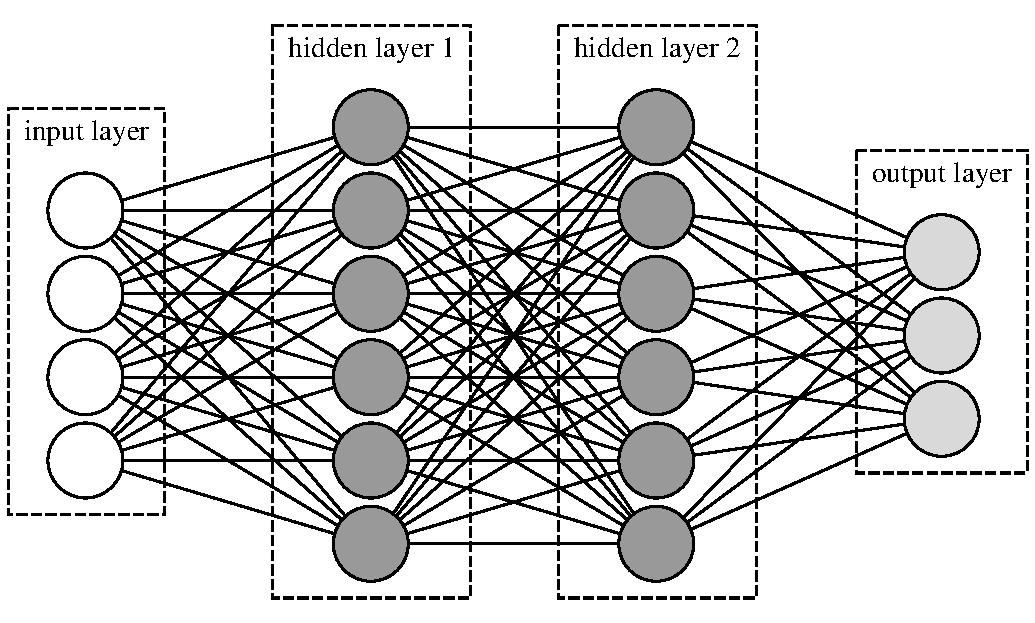
\includegraphics[width=0.8\textwidth]{graph}
  \caption{A fully connected feed-forward neural network with four input
  nodes, two hidden layers, and three output nodes.}
  \label{fig:mlp-diagram}
\end{figure}

The ``vanilla'' neural network is the feed-forward network, also known as the
\ac{MLP}. This model incorporates one or more
hidden layer in-between the input layer (the feature vector) and the output
layer. A diagram of an example \ac{MLP} with two hidden layers can be seen in
figure \ref{fig:mlp-diagram}. For multi-class prediction, the output layer
typically uses a \emph{softmax} activation. This has the property of
restricting each output value to be in the interval $(0,1)$, and additionally
makes sure all output values sum to $1$. These properties allow the outputted
values to be interpreted as a probability distribution.

\begin{equation}\label{eq:softmax}
  \mathrm{softmax}(x)_i = \frac{\exp{x_i}}{\sum_{j=1}^{m}\exp{x_j}}
\end{equation}

\subsection{Convolutional neural networks}

\acp{CNN} can exploit local patterns in the input, unlike the \ac{MLP}, which
has no way to identify elements of the input layer as being ``close'' to each
other in any sort of measure. \acp{CNN} use convolutional layers to make
these local relationships explicit.

\acp{CNN} are widely employed in image processing models, using
two-di\-men\-sional convolutional layers. These models can often get very
deep, using a number of convolutional layers at different levels in the
network, interspersed with pooling or downsampling layers.

There are also \ac{NLP} applications where \acp{CNN} can be employed. Unlike
images, data in \ac{NLP} is usually sequential or one-dimensional, but it may
be converted into two dimensions, for example by replacing each word by an
embedding vector.


\subsection{Recurrent neural networks}
\label{seq:rnn}

\acp{RNN} are suited to sequential data. They make have an internal
\emph{state} that is passed between time steps. A benefit of \acp{RNN} is
that they can accept input of any length and also produce sequential output
of any length. This in contrast to feed-forward neural networks, which take a
fixed-length vector as their input.

A long standing problem in training \acp{RNN} was that when applying
backpropagation through time, the gradient values can tend toward zero or
diverge because of multiplication across many time steps. This is known as
the \emph{vanishing} and \emph{exploding gradients problem}, respectively.
Mitigation techniques include replacing the units of the network with what's
known as \emph{gated units}, that are especially designed to address these
problems. \acp{GRU} and \acp{LSTM} are widely used gated units in RNNs. The
`gates' in these network are what enables the cell to keep information in
working memory over longer spans of time without succumbing to the problem of
vanishing or exploding gradients.

The equations in \ref{eq:lstm} define the LSTM cell. It computes three gates
named $i$, $f$ and $o$, which are vectors with values between 0 and 1. The
GRU cell, defined by the equations in \ref{eq:gru}, is slightly simpler. It
computes only two gates, named $z$ and $r$. The $\sigma$ activation function
can be a number of functions $\sigma : \mathbb{R} \rightarrow [0, 1]$, and is
commonly the sigmoid (Eq. \ref{eq:sigmoid}) or hard sigmoid (Eq.
\ref{eq:hardsigmoid}) function.

\begin{equation} \label{eq:hardsigmoid}
  \sigma(x) = \begin{cases}
    0                 & : x < -2.5 \\
    0.2 \cdot x + 0.5 & : -2.5 \leq x \leq 2.5 \\
    1                 & : x > 2.5
  \end{cases}
\end{equation}

\begin{gather} \label{eq:lstm}
  \begin{split}
  s_j = R_{\text{LSTM}}(s_{j-1}, x_j) &= [c_j;h_j] \\
                           c_j &= f \odot c_{j-1} + i \odot z \\
                           h_j &= o \odot \tanh(c_j) \\
                             i &= \sigma(x_j W^{xi} + h_{j-1} W^{hi} + b_i) \\
                             f &= \sigma(x_j W^{xf} + h_{j-1} W^{hf} + b_f) \\
                             o &= \sigma(x_j W^{xo} + h_{j-1} W^{ho} + b_o) \\
                             z &= \tanh(x_j W^{xz} + h_{j-1} W^{hz} + b_z) \\
          O_{\text{LSTM}}(s_j) &= h_j
  \end{split}
  \\[2ex]
  s_j\in \mathbb{R}^{2d_h}, x_i\in \mathbb{R}^{d_x},
  \left\{c_j, h_j, i, f, o, z, b_{\circ}\right\}\subseteq \mathbb{R}^{d_h},
  W^{x\circ}\in \mathbb{R}^{d_x\times d_h},
  W^{h\circ}\in \mathbb{R}^{d_h\times d_h} \notag
\end{gather}

\begin{gather} \label{eq:gru}
  \begin{split}
  s_j = R_{\text{GRU}}(s_{j-1}, x_j) &= (1 - z) \odot s_{j-1} + z \odot {\tilde s}_j \\
                            z &= \sigma(x_j W^{xz} + h_{j-1} W^{sz} + b_z) \\
                            r &= \sigma(x_j W^{xr} + h_{j-1} W^{sr} + b_r) \\
                 {\tilde s}_j &= \tanh(x_j W^{xs} + (r \odot s{j-1}) W^{sg} + b_z) \\
          O_{\text{GRU}}(s_j) &= s_j
  \end{split}
  \\[2ex]
  x_i\in \mathbb{R}^{d_x},
  \left\{s_j, {\tilde s}_j, z, r, b_{\circ}\right\} \subseteq \mathbb{R}^{d_s},
  W^{x\circ}\in \mathbb{R}^{d_x\times d_s},
  W^{s\circ}\in \mathbb{R}^{d_s\times d_s} \notag
\end{gather}


\subsection{Natural language features}

For applications of machine learning in \ac{NLP}, we often want to use the
words in a document as features. However, the vast number of different words
in a language can lead to inefficient use of memory and computing power if
the words are represented naively, for instance with a one-hot vector
encoding with the vector having the number of dimensions equal to the size of
the lexicon. It is therefore useful to map words to a lower-dimensional
representation, known as an \emph{embedding}.

\sloppy Training embeddings rely on the distributional hypothesis, namely
that words with similar meanings are likely to appear in similar contexts.
Therefore, without prior knowledge of any words in a language, the resulting
embeddings are likely to put words with similar meanings close to each other
in the embedding space. It has also been observed that semantic relations
between words, for instance regarding gender or inflection, corresponds to
defined directions in the embedding space\autocite{mikolov2013linguistic}.
These relations can be found by subtracting word vectors. A famous example of
an emergent analogy learned by the embeddings is: ``Man is to king as woman
is to ...''. In terms of arithmetic on embedding vectors, the embeddings
modelled the analogy as $\vec{king}-\vec{man}+\vec{woman}\approx\vec{queen}$.
\fussy

There exists a number of embedding models, including Word2Vec
\autocite{mikolov2013word2vec} and GloVe \autocite{pennington2014glove}.
These models can be used to compute embeddings based on new training data, or
one may use pre-trained embeddings.

Different approaches to embeddings may be necessary for different languages.
A word-based approach can work well for a relatively analytic language such
as English, but might be less suited for agglutinative or synthetic
languages, because of the differing amount of semantic information present in
a single token. A converse problem occurs where a sequence of words is best
analyzed as a single unit.

Another issue is ambiguity, as the process of training embeddings only
considers the form of a word. Homographs like \emph{well}, which can be both
an adverb and a noun, are each mapped to a single embedding vector, with no
way to distinguish the different meanings of the word.

It is also possible to embed \ngrams of characters instead of words. A
disadvantage of this approach is that it becomes more difficult to
distinguish words with similar spelling, but different meaning, and it does
not solve the problem of homographs. However, it seems that the embeddings
may still be more robust when encountering spelling mistakes. The embeddings
based on word forms will see ``beautiful'' and ``beutiful'' as completely
separate words, while there still exists similarities between them on the
level of characters: they share a good portion of their \ngrams. Another
advantage might be the possibility of accessing semantic meaning at a
sub-word level, including prefixes and suffixes.

For representing a document non-sequentially, a common approach is to use
\ac{CBOW}. This is the sum or average of embedding vectors for all active
features \autocite[352]{goldberg2016primer}. \ac{CBOW} thus disregards some
information, including order and whether features occur close to each other
in the document.


\subsection{Multi-task learning}

Multi-task learning refers to optimizing a target function for two or more
different tasks simultaneously \autocite{ruder17overview}. One benefit of
this approach is increased generalization. Intuitively, this is feasible
because the neural network needs to find a representation which is useful for
all the tasks it is optimizing on, and thus is less likely to pick up noise
in the data than it might be when only considering a single task. A
representation that is useful to different tasks is more likely to be able to
generalize, not only to data beyond the training data, but to new tasks which
were not part of the training process as well.

In practice, for neural networks, the tasks in question share some of the
inner layers of the network, but have separate output layers. This is called
parameter sharing. Another approach is to keep different parameters for each
of the tasks, but add a regularization loss that prevents the parameters from
diverging too much from each other. The output layers are not necessarily at
the same depth. A low-level auxiliary task can have its output layer rather
early while the main task uses more hidden layers. In the backwards pass,
losses at all the output layers should be minimized.

\textcite{ruder17} lists several tasks in natural language processing that
have been subject of experiments with multi-task learning, including machine
translation, speech recognition, semantic parsing and chunking. These tasks
have been jointly trained with auxiliary tasks such as predicting the next
word, recognizing phonemes, part-of-speech tagging, and more. Among others,
the author cites \textcite{pappas17}, who used multi-task learning to train a
document classifier using 8 different languages, sharing parameters between
the models for different languages. The model they used for this was a
hierarchical attention network.

\textcite{alonso17} investigated the effect of different auxiliary tasks and
combinations of these on a \ac{LSTM} recurrent network for sequence labelling
tasks. The main tasks they considered in the study were labelling semantic
frames, semantic supersenses, named entity recognition, ontological types for
senses and Multi-Perspective Question Answering.

They used an auxiliary task called \textsc{FreqBin}, whose objective is to
predict the log frequency of a word, discretized into a number of bins. This
study tried a new binning strategy which improved the utility of
\textsc{FreqBin} as an auxiliary task compared with previously examined
strategies. While the previous variants took the logarithm of the token's
frequency in a chosen base and rounded down to the nearest integer, the new
strategy ranked all tokens by frequency grouped them into labels by a given
quantile. In the study, they used $k=5$, yielding 5 \textsc{FreqBin} labels
with the same number of examples each.


\section{Learner language}

In the linguistic field of \ac{SLA}, linguists have described characteristics
of the language of people who are learning a second language. It is common to
refer to a person's first language(s), that is the language(s) they learned
when they first started to speak, as L1, and any languages acquired later in
life as L2. Since language acquisition is a gradual process, we can speak of
an \emph{interlanguage}, which is an idiolect with systematic rules belonging
to the learner in question, but which is different from their target
language. Interlanguage is not stable, but changes as part of a learner's
acquisition process \autocite[358]{myers-scotton}.

Interlanguage can show influences from the learner's L1 in several respects,
for instance intonation and produced phonemes in pronunciation, syntactic
mistakes like inflection and word order, or even the literal translation of
idioms that do not exist in the same form in the target language. The study
of linguistic \emph{transfer} is an attempt to understand these influences.


\subsection{Automated assessment}

\acf{AES}, in the literature also referred to as Assessment of proficiency or
automated text scoring (ATS), considers the task of assigning a grade to a
free form text, often responding to a specific prompt. The task can apply to
texts written in either a first or a second language. In many settings, we
can expect that documents may be written in either a first or a second
language. This is the case for instance in tests given in schools, where some
pupils may come from a minority language background. \ac{AES} can be framed
as a supervised learning task, using a corpus of texts that have each been
labelled with a score or a proficiency rating.

Automating the assessment task can benefit applications in language
education. People learning a new second language will benefit from feedback
as to which proficiency level they might be on, for instance in relation to
the \ac{CEFR}. This may help people who want to take language
examination to find the appropriate timing and level of testing, since an
examination can be both an economical and logistical inconvenience.
Automation also allows students to receive feedback quicker and more
frequently.

Previous work by \textcite{vajjala17} uses the TOEFL11 corpus of non-native
English \autocite{blanchard13} and the First Certificate of English (FCE)
corpus \autocite{yannakoudakis2011new}. This study examines which features
may be most informative in relation to the task, and whether these are the
same features for different datasets. \citeauthor{vajjala17} uses a number of
linguistic features for the task, including several different measures for
the lexical diversity, distribution of \ac{POS} tags, and
syntactic complexity. The models in the study utilize up to 116 different
features. Applied pre-processing includes syntactic parsing of sentences in
order to extract features from the parse trees. These syntactic features
include measures of average sentence length, clauses per sentence, the height
of the parse tree etc. Several of these features were based on previous work
on measuring syntactic complexity in L2 writing by
\textcite{lu2010automatic}.

Other features are designed to capture discourse properties of the text,
based on reference chains. The English language has different ways of
referring to previous information in a discourse, which is a core element of
fluent language use. For instance, the definite/indefinite distinction is a
way to reference previous information in English. This is not the case
cross-linguistically, so features like this are language-specific.
\citeauthor{vajjala17}'s features are measures of the proportions of
different pronoun types, determiners and definite noun phrases, and more, in
a reference chain, along with the average length of a reference chain.

Notably, the author did not use word or \ac{POS} \ngrams as features in the
study. The reasons given for this is that the sparse nature of \ngram
features make them hard to interpret, and they can introduce topic bias to
the model. The essays are written on different topics, making it likely that
certain words indicate the topic of an essay. \ngrams can model errors
relative to the learner's target language, but she already uses features
designed to model this. Nor are character \ngrams used as features here,
though they are generally widely used in a various NLP applications.
\citeauthor{vajjala17} also experimented with using the writing prompt and
the native language (L1) of the text's author as features.

The author trained a number of different models using different subsets of
the features. All models are linear classifiers trained with the Sequential
Minimal Optimization algorithm, a variant of support vector machines. The
model that achieved highest accuracy in the study was one that incorporated
all the features, yielding an accuracy of 73.2\% on TOEFL11. Removing the
prompt and L1 as features resulted in a tiny drop in accuracy down to
73.0\%.

The length of the text turned out to be one of the most informative features
in both the datasets used. However, text length correlated positively with
proficiency on TOEFL11, but negatively on the FCE corpus.


\subsection{Native Language Identification}

\ac{NLI} is the task of predicting the native language of an author based on
a text written in one of the author's \acp{L2}. The task is
dependent on systematic differences between interlanguages for learners with
the same target language, but different L1s. The feasibility of this task
proves intrinsically that these systematic differences exist, as linguists
studying transfer try to explain.


\subsubsection{Shared tasks in NLI}

\ac{NLI} has been the subject of three shared tasks, in 2013
\autocite{tetreault2013report}, 2016 \autocite{schuller2016interspeech} and
2017 \autocite{nli17}. The 2013 shared task used only written documents,
whereas the 2016 shared task was audio data only. Lastly, the latest shared
task in 2017 contained both written and spoken documents. Teams participating
in 2017 could choose between three tracks corresponding to written data only,
spoken data only, or both. Only teams participating in the first track, using
written data only, are considered below.

The written documents in the task was English L2 essays, written by learners
with 11 different L1s. The best-performing system in the track using only
written essays had a macro-averaged \FI score of $0.8818$, using stacked
classifiers combining logistic regression on sentences with a \ac{SVM}
meta-classifier \autocite{cimino17}.

The best performing team which used neural networks was \textcite{li17}, who
used a multi-layer perceptron meta-classifier to combine outputs from
\ac{SVM} base classifiers, and reported a \FI score of $0.8654$. Another team
experimented with different neural network architectures, including \acp{RNN}
and a \ac{CNN} variant known as a deep residual network
\autocite{bjerva2017neural}. Their best result was with a stacked model,
combining their different models with an \ac{SVM} meta-classifier. Their best
ensemble model achieved a \FI score of $0.8323$, and used no external
resources, i.e. no pre-trained embeddings.


\subsubsection{NLI for Norwegian}

While the shared tasks have been English learner language only, there exists
studies using different corpora with other target languages, among them
Norwegian. Norwegian \ac{NLI} has been attempted by \textcite{malmasi15},
using the ASK corpus \autocite{tenfjord06}. In their methodology, they create
artificial documents to train on by segmenting the learner texts into
sentences, then putting all the sentences from learners with the same L1 into
a bag and sampling sentences from the bag to create the new documents. Their
rationale for the methodology is that all the resulting documents are of
similar length, and that they eliminate the variation between individual
writers that otherwise might present a stronger signal than the writer's L1
alone.

In a later study \autocite{malmasi17}, they perform an \ac{NLI} experiment on
several corpora, namely TOEFL11, the Norwegian ASK corpus and the Jinan
Chinese Learner corpus. However, they were not able to utilize the same
features for all the different corpora. For Norwegian, they only use the
features \emph{function word unigrams}, \emph{function word bigrams} and
\emph{part-of-speech \ngrams}. For the English corpus, they were able to use
other features such as dependencies and context free grammar-rules. By
combining a selection of base classifiers using a \ac{LDA} meta-classifier
trained with bootstrap aggregation (bagging), they achieve an accuracy of
$0.818$ on the Norwegian corpus.

They reapply the above methodology of generating artificial essays for the
Norwegian and Chinese corpora. In particular, they mention that this removes
bias stemming from different topics. In the case of the TOEFL11 corpus,
however, the authors of the corpus have made an effort to make the documents
balanced in terms of both L1 and the writing prompt which the learner has
answered.

Adopting this methodology, however, does mean letting go of the discourse
properties of a text, which could offer valuable cues both toward the L1, and
in relation to the automated assessment task. Moreover, it does not reflect
realistic real-world documents, which in many cases are written by
individuals, and contain bias toward specific topics.


\subsection{Datasets}

Several available datasets for different languages have been or can be used
in the tasks discussed above. Desirable properties for these tasks include
representing a broad selection of different language backgrounds and
proficiencies, a balanced selection with respect to variables such as L1 and
topic, and rich metadata. Below we will look at two corpora with English and
one with Norwegian learner texts. There exists learner corpora for several
other target languages as well, including Chinese and Czech.


\subsubsection{TOEFL11}

The TOEFL11 corpus was presented in 2013 and was specifically designed to be
suitable for the \ac{NLI} task \autocite{blanchard13}. The documents are
essays from the English proficiency test TOEFL, which many take as
preparation for admission to higher education in English-speaking countries.
The corpus contains metadata for the writers' L1s and the proficiency level
their essay was assessed to. The proficiency levels are specific for the
corpus and correspond to low, medium and high proficiency, without reference
to external frameworks such as \ac{CEFR}. The represented language
backgrounds are Arabic, Chinese, French, German, Hindi, Italian, Japanese,
Korean, Spanish, Telugu, and Turkish. The datasets for the \ac{NLI} shared
tasks in 2013 and 2017 (the written essays) were extracted from TOEFL11.

The corpus contains 1100 essays per L1, in total 12,100 essays. The average
word count for the essays is 348, so in total the corpus contains more than
4,210,000 words.


\subsubsection{FCE}

This corpus was first introduced by \textcite{yannakoudakis2011new}. It is a
subset of the Cambridge Learner Corpus, containing the documents that were
collected from the First Certificate of English test. It contains 1238
documents, each containing a written response to two different tasks. The
documents are marked on a proficiency scale from 1 to 40.


\section{Conclusion}

The thesis will be focused on training an automated essay scoring model on
Norwegian data using multi-task learning. Native language identification is
one of possibly more auxiliary tasks that will be attepted.
